\documentclass[class=../report, crop=false]{standalone}
\usepackage{graphicx}
\usepackage{tabularx}
\usepackage{pgfplots}
\usepackage{pgfplotstable}

\begin{document}

\section{Evaluation}

We began the evaluation process by \gls{winnow} our \gls{conceptfrags} based on feasibility, requirements and \gls{techready}; any concepts containing the eliminated fragments were winnowed immediately.
\gls{wholeconc} were ranked using a \gls{pugh}.
The process was repeated with a second \gls{datum} to ensure accurate ranking.
We advanced the four best concepts to scoring where we used multiple prototype tests and a \glsdisp{wdm}{WDM} to select the best design.

\subsection{Winnowing}

We established our \gls{winnow} criteria based on the requirements of the Rail-Rider locomotive.
We decided to \glsdisp{winnow}{winnow} the \gls{conceptfrags} individually to expedite the process due to our time restriction and large number of concepts.
The independent nature of our \gls{conceptfrags} made this process viable.
Many of the creative concepts were eliminated due to feasibility issues or requirement violations\footnotemark.
\footnotetext{See Appendix \ref{app:winnowing}: \nameref{app:winnowing} Table \ref{app/table:energytomech}--\ref{app/table:connectcart}}
We winnowed the full concepts and discarded any designs containing the eliminated concept fragments\footnotemark.
\footnotetext{See Appendix \ref{app:winnowing}: \nameref{app:winnowing} Table \ref{app/table:concwinnow1}--\ref{app/table:concwinnow3}}
We noticed that some concepts were very similar, so we combined the best features between them to create an improved \gls{wholeconc}.
All remaining concepts were advanced to ranking.

\clearpage

\subsection{Ranking}

We advanced eight concepts to ranking where we used a \gls{pugh} to compare their performance.
In order to reduce the time spent on ranking, we used qualitative assessments of each design to complete the \gls{pugh}.
Our evaluation method for each criteria is described in Table \ref{table:winnowingcriteria}.

\begin{table}[H]
	\centering
	\small
	\begin{tabular}{l | l}
		\textbf{Criteria} & \textbf{Qualitative Assessment} \\ \hline
		Aesthetics & Any remarkable, visual differences \\
		Energy & Number of electrical components \\
		Cost & Rough estimate of most expensive parts eg. gear trains and motors (intuition based) \\
		Acceleration & Torque to mass ratio \\
		Torque & Number of motors and best gear ratio \\
		Stability & Based off performance of the type of wheel (Cylindrical vs Conical)\\
	\end{tabular}

	\caption{Winnowing Criteria Description}
	\label{table:winnowingcriteria}
\end{table}

Our \gls{pugh}\footnotemark favoured six concepts of the eight evaluated.
\footnotetext{See Appendix \ref{app:pugh}: \nameref{app:pugh} Figure \ref{app/table:pughsimplicity1}--\ref{app/table:pughsimplicity2}}
We repeated the process using a second \gls{datum} to test the differences between only the top-performing designs.
The results of second \gls{pugh}\footnotemark showed that four designs were consistently outperforming the others.
\footnotetext{See Appendix \ref{app:pugh}: \nameref{app:pugh} Figure \ref{app/table:pughpuff}}
We decided to advance only these four concepts to further testing and scoring.

\clearpage

\subsection{Prototype testing}

We conducted several \gls{prototype} tests to gather enough evidence to properly score the remaining concepts.
We tested the cornering ability of conical and cylindrical wheels using a qualitative test\footnotemark.
\footnotetext{See Appendix \ref{app:prototypetests}: \nameref{app:prototypetests} Table \ref{app/table:wheeltest}}
The test demonstrated that the \gls{conical} have greater cornering ability particularly when the chassis has a low centre of gravity.
We decided to move forward with the \gls{conical} design.

Our team attempted to maximize the \glsdisp{friction}{frictional} force experienced by the driven wheels on our train; not only would this allow us to pull more cargo, but it would also let us accelerate faster and turn better.
We tested the coefficient of static \gls{friction} of \glsdisp{pla}{PLA filament}, rubber plasti-dip, and elastic bands in order to optimize the friction of our wheels\footnotemark.
\footnotetext{See Appendix \ref{app:prototypetests}: \nameref{app:prototypetests} Table \ref{app/table:staticcoeff}}
The elastic bands were chosen over the plasti-dip due to their more durable nature; the plasti-dip wore off after a short amount of testing (Figure \ref{fig:wheelcoating}).
We also distributed our weight closer to the driven \glsplural{axle}; this would serve to further increase frictional force by increasing the normal force on those wheels.

\begin{figure}[H]
	\centering
	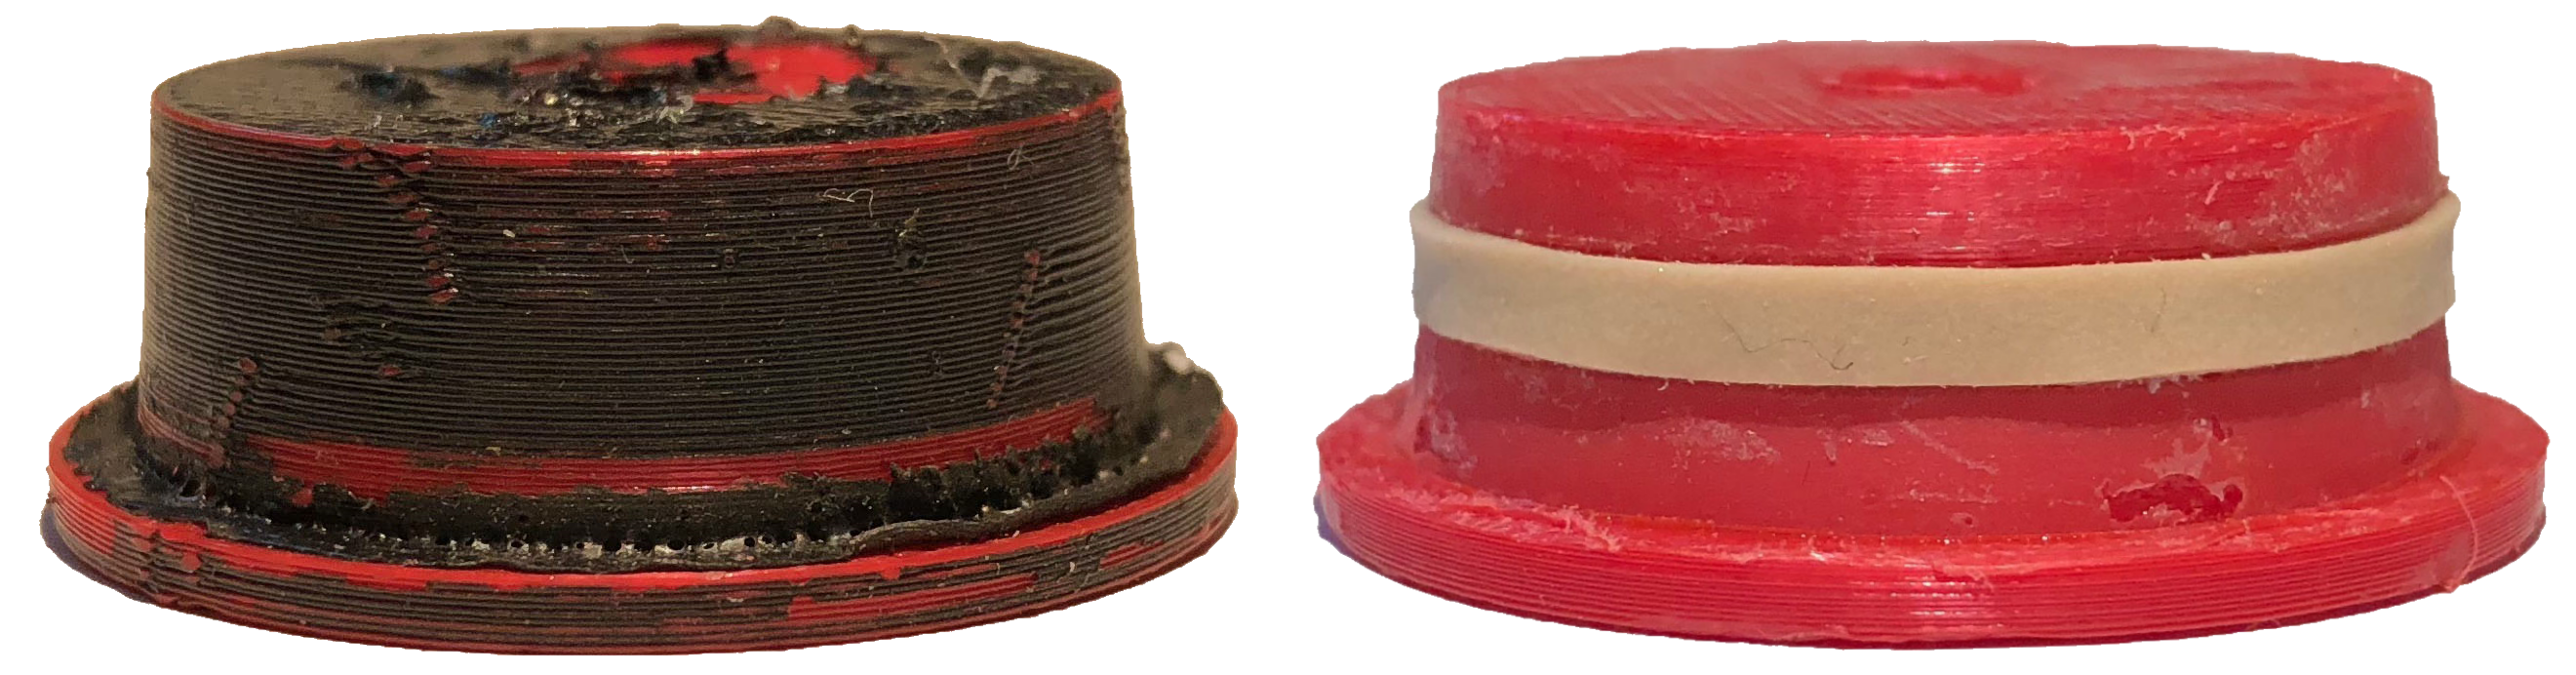
\includegraphics[width=0.7\textwidth]{../res/img/wheelcoating}
	\caption{Wheel Coating Test of Durability}
	\label{fig:wheelcoating}
\end{figure}

Our best concepts used a gear or pulley transmission to transfer \gls{torque} to the wheels.
We tested the \gls{torque} output by determining the largest angle each design could climb without stalling.
We completed calculations\footnotemark comparing a two motor system with a single motor gear train.
\footnotetext{See Appendix \ref{app/sub:dualdrivetorque}: \nameref{app/sub:dualdrivetorque}}
The results of these tests indicated that a dual driven gear transmission system was the most effective at transferring \gls{torque}.

The \gls{pulleydrive} had many issues during testing.
The distance required to create enough tension for the system to operate spanned over half of our vehicle length which invalidated a variable pulley drive.
The belt slipping or the motor stalling occured, producing enough heat to soften the \gls{pla} and left the pulley susceptible to falling off of the motor’s \gls{axle} and to rapid wear from the belt (Figure \ref{fig:pulleytest}).

\begin{figure}[H]
	\centering
	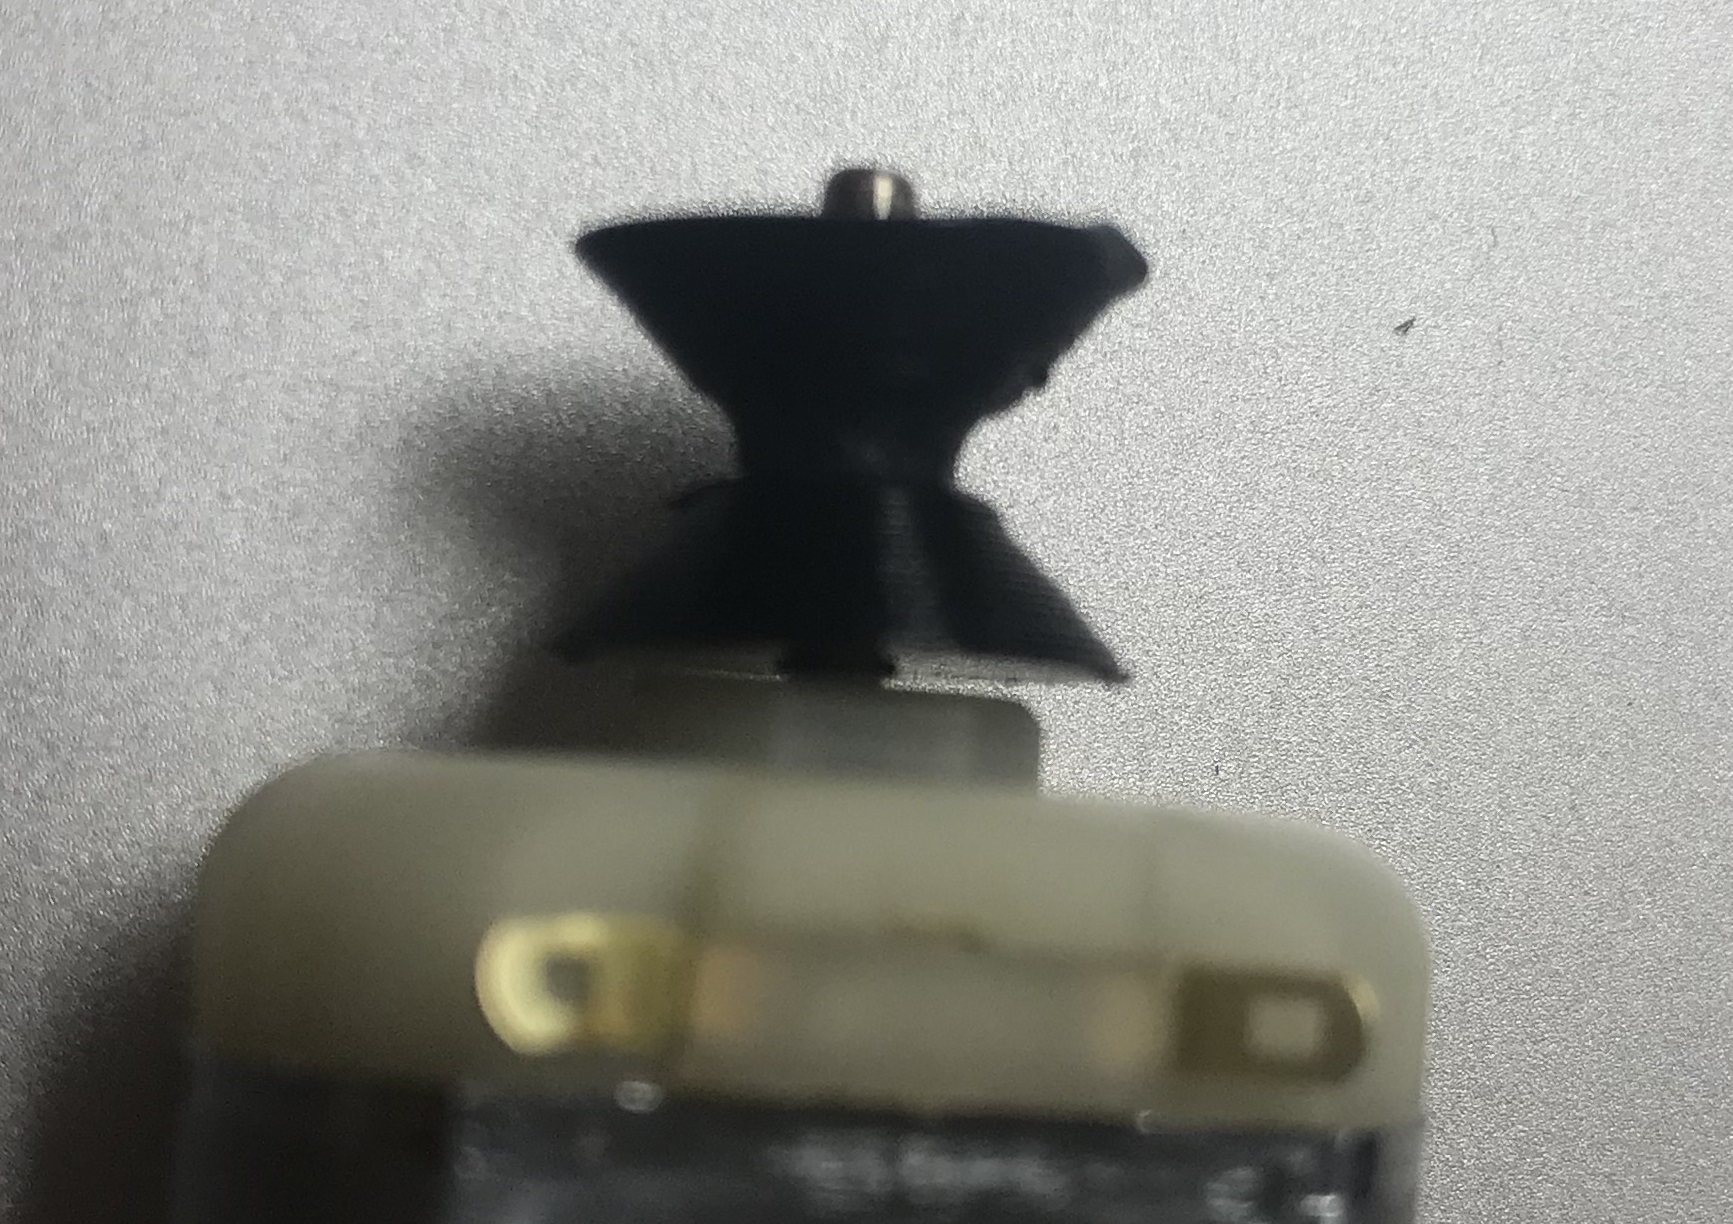
\includegraphics[width=0.7\textwidth]{../res/img/pulleytest}
	\caption{Wear on V-shape pulley}
	\label{fig:pulleytest}
\end{figure}

Our team opted for the variable gear drive due to the belt drive’s problematic nature.
Although, the possibility of stalled motors exists in the gear train option, the gear ratio prevents this from happening at smaller angles, making this unlikely during the competition.
As an added precaution, we fitted grub screws with nuts to better connect the gear to the axle.

\clearpage

We generated a computer simulation of the train going around the track in each round.
The model (Figure \ref{fig:trainsim}) indicated that the train would continue to increase in speed well above our tipping velocity\footnotemark.
We decided to create a braking system to solve this problem.
\footnotetext{See Appendix \ref{app/sub:tracksimulation}: \nameref{app/sub:tracksimulation}}

\begin{figure}[H]
	\centering
	\begin{tikzpicture}
		\begin{axis}[
				title={\textbf{Simulation for Round 2}},
				width=0.8\textwidth,
				height=0.45\textwidth,
				grid=major,
				ytick distance=0.5,
				xmin=0,
				xlabel={Position on Track (m)},
				legend style={
					at={(1.1,0.5)},
					anchor=west,
					nodes={
						scale=0.8, transform shape
					}
				},
				legend image post style={mark=none}
			]
			\addplot table [x=x, y=v, col sep=comma,mark=none]{trainsim.csv};
			\addplot table [x=x, y=a, col sep=comma,mark=none]{trainsim.csv};
			\addplot table [x=x, y=tip, col sep=comma,mark=none]{trainsim.csv};
			\legend{Velocity (m/s), Acceleration (m/s\textsuperscript{2}), Tipping Velocity (m/s)}
		\end{axis}
	\end{tikzpicture}
	\caption{Simulation model}
	\label{fig:trainsim}
\end{figure}

We tested a \gls{photores} to determine its sensitivity to difference in colour changes.
The photoresistor was accurate at differentiating between the table and track rungs across multiple trials and remained accurate at higher speeds\footnotemark.
\footnotetext{See Appendix \ref{app/sub:photores}: \nameref{app/sub:photores}}
We implemented this to determine our position on the track and when to begin braking.

\clearpage

\subsection{Weighted Decision Matrix}

Using the results of our prototype tests, we scored our remaining designs in a WDM.
We evaluated the concepts based on cost, energy, derailment stability, cargo transfer ability, and risk.
Our complete WDM can be found in Appendix \ref{app:wdm}: \nameref{app:wdm}
We determined that the dual drive design, Get Hitched, was the best.
A summary of the scores is shown in Figure \ref{fig:wdm}.

\pgfplotstableread[col sep=comma]{wdm.csv}{\wdmdata}
\pgfplotstablegetcolsof{\wdmdata}

\begin{figure}[H]
	\centering
	\begin{tikzpicture}
		\begin{axis}[
				width=0.8\textwidth,
				height=0.6\textwidth,
				reverse legend,
				ybar stacked,
				bar width=15pt,
				ymin=0,
				xtick=data,
				xticklabels from table={\wdmdata}{concept},
				ymajorgrids,
				legend style={
					at={(1.05,0.5)},
					anchor=west,
					nodes={
						scale=0.8, transform shape
					}
				},
				legend image post style={mark=none}
			]
			\addplot table [x expr=\coordindex, y index=1]{\wdmdata};
			\addplot table [x expr=\coordindex, y index=2]{\wdmdata};
			\addplot table [x expr=\coordindex, y index=3]{\wdmdata};
			\addplot table [x expr=\coordindex, y index=4]{\wdmdata};
			\addplot +[
				point meta=y,
				nodes near coords,
				every node near coord/.append style={
					black,
					fill=white,
					fill opacity=0.75,
					text opacity=1,
					outer sep=\pgflinewidth,
				}
			]table [x expr=\coordindex, y index=5]{\wdmdata};
			\legend{Competition Cost, Energy, Derailment Stability, Cargo Transfer Ability,Risk}
		\end{axis}
	\end{tikzpicture}
	\caption{Simulation model}
	\label{fig:wdm}
\end{figure}

Limitations in space made producing two gear trains with sufficient gear ratios very difficult.
We combined Puff with Get Hitched to create a design with a singular gear transmission driven by two motors.
We could therefore utilize the positive aspects of the variable gear train as well as the strong attributes of Get Hitched.

\end{document}
